One of the most important things when optimizing CUDA code is optimizing the memory access done by the kernel which is being executed. The CUDA GPU memory model, which is described in depth in \cref{sec-hw-memory-model}, contains five levels of memory going from smallest and fastest to largest and slowest, \texttt{Registers}, \texttt{Shared Memory}, \texttt{Level 1 Cache}, \texttt{Level 2 Cache} and \texttt{Global Memory}. While all of these should be kept in mind, while optimizing a CUDA program, it can be seen in \cref{sec-pm-memory} in the chapter describing the programming model, that when programming, there is only four type of memory to be concerned with, \texttt{Host Memory}, \text{Global Memory}, \text{Shared Memory} and \texttt{Local Memory}.\\
To optimize global memory access another concept needs to be introduced, which is coalesced memory. Where the indication for the memory here is that coalesced memory is memory, which is closely related, thereby placed next to each other when looking at the address space of the memory. When threads in each streaming multiprocessor are divided into Warps (SIMT Units), as discussed in \cref{sec-hw-warps-threads}, the Warp, as they are SIMT, are also in charge of issuing memory reads and writes. The Warp here attempts to issue global memory access into as few transactions as possible to minimize DRAM bandwidth. This, in turn, means that to optimize memory access, we have to have threads access memory, which is in the address space is next to each other. In turn, this also increases performance as the Warp will not have to issue reads or writes for a single thread out of the 32 threads contained within a Warp.\\

\begin{figure}[ht]
	\centering
	\fbox{
		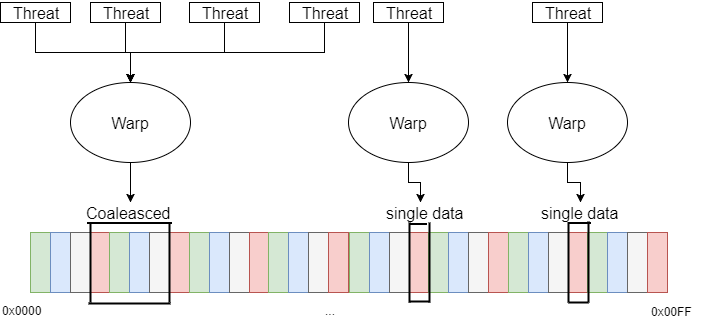
\includegraphics[width=0.9\textwidth]{figs/opti/coalesed_memory.png}
	}
	\caption{Example of coalesced memory access vs random memory access, where other threads are idle while the warp is accessing memory.}
	\label{fig:coalesced_memory}
\end{figure}

\Cref{fig:coalesced_memory} show how multiple threads being in the same warp, accesses coalesced memory. The reason for coalesced memory being important is that single data access is often just as expensive in time as it is to access larger pieces of data. This is because memory is only read in chunks, which correlates to a single read being able to supply multiple threads with data or a single threat with a large amount of data of which there is no guarantee that it uses all of.\\

However, it is very difficult to avoid all random memory access, which is where our memory model become important, as different levels of memory are available for use. Instead of using the slower \texttt{Global memory}, \texttt{Shared memory} can be used for the random memory access. This can be accomplished by using shared memory as a buffer. As shared memory is faster, these memory accesses will also be performed faster. As an example of the optimization gain, we can take a look at two different reduce kernels, one which does direct access to global memory, and one which makes use of shared memory. The code for the reduce kernel without any optimization can be found in listing \ref{lst:reduce_kernel}.\\

Using the kernel to sum 2048 elements, a runtime could be measured. To get a more precise measurement, the kernel was run a thousand times on the same elements, thus calculation an average runtime of 0.971 ms. To optimize the before mentioned reduce kernel, shared memory was used internally in the kernel, the code can be seen in listing \ref{lst:reduce_shared}.

\begin{lstlisting}[language=C,caption={Optimized reduce kernel, using shared memory},label=lst:reduce_shared]
__global__ void reduce_kernel_shared(unsigned *in, unsigned *out) 
{
	auto id = blockDim.y * blockDim.x * blockIdx.x + threadIdx.y * blockDim.x + threadIdx.x;
	__shared__ int sdata[K/2];
	sdata[id] = in[id * 2] + in[id * 2 + 1];
	for(size_t i = 1 ; i< K/2; i *= 2) 
	{
		if (id % (2 * i) == 0)
			sdata[id] += sdata[id + i];
		__syncthreads();
	}
	if (id == 0) 
		out[0] = sdata[0];
}
\end{lstlisting}

Performing the same measurements as before, an average runtime of 0.831 ms was calculated. And while this performance difference may not seem very significant it is still an improvement, and running the kernel on a larger array then 2048 elements, might give even further improvements.\\

In the end, memory optimization is some of the best ways to gain improvements in performance with CUDA programs, however like most optimization is difficult, and often gives less performance per hour spend than other things, such as picking a better algorithm as described in \cref{sec-general-opti}. That being said, the core terms explained in this section, being coalesced memory and shared memory, can for some algorithms be fairly simple to implement.